\documentclass[twocolumn]{article}
\usepackage{hyperref}
\usepackage[pdftex]{graphicx}
\usepackage{listings}
\usepackage{footnote}
\usepackage{float}

\hypersetup{%
  pdfborderstyle={/S/U/W 1}% border style will be underline of width 1pt
}

\title{Using Microsoft Visual Studio}
\author{CS 104 Teaching Team}
\date{}

\begin{document}
\graphicspath{ {./images/} }
\maketitle
\paragraph{Introduction} This guide is intended to get you familiarized with C++ programming using an integrated development environment (IDE). Microsoft Visual Studio\footnote{\url{http://www.microsoft.com/visualstudio/eng/products/visual-studio-express-for-windows-desktop}} has core project creation features including a code editor, debugger, and designer.

\section{Microsoft Visual Studio}
\subsection{Overview} Visual Studio is a program that allows you to write, edit, compile, and debug code in a broad range of programming languages. It is an Integrated Development Environment, which allows programmers to create a variety of projects, including user interface applications and websites. For the purposes of this class and this guide, we will focus on the basic usage of Visual Studio to create console programs using C++. 

\subsection{Creating a Project in Visual Studio}	For this exercise, we will be printing out the phrase, “Hello World!” To begin writing a program in Visual Studio, you must first create a new project.
\begin{enumerate}
	\item At the top left corner, click \texttt{File}. Select \texttt{New}, and then select \texttt{Project}. A dialog box will appear.
	\item In the left pane of the dialog box, click on \texttt{Win32} under the Visual C++ section.
	\item Select the Win32 Console Application option, and name your project. You can name it anything, but remember to keep it simple and easy to remember (e.g. “Hello World”)
	\begin{figure}[htbp]
		\centering
		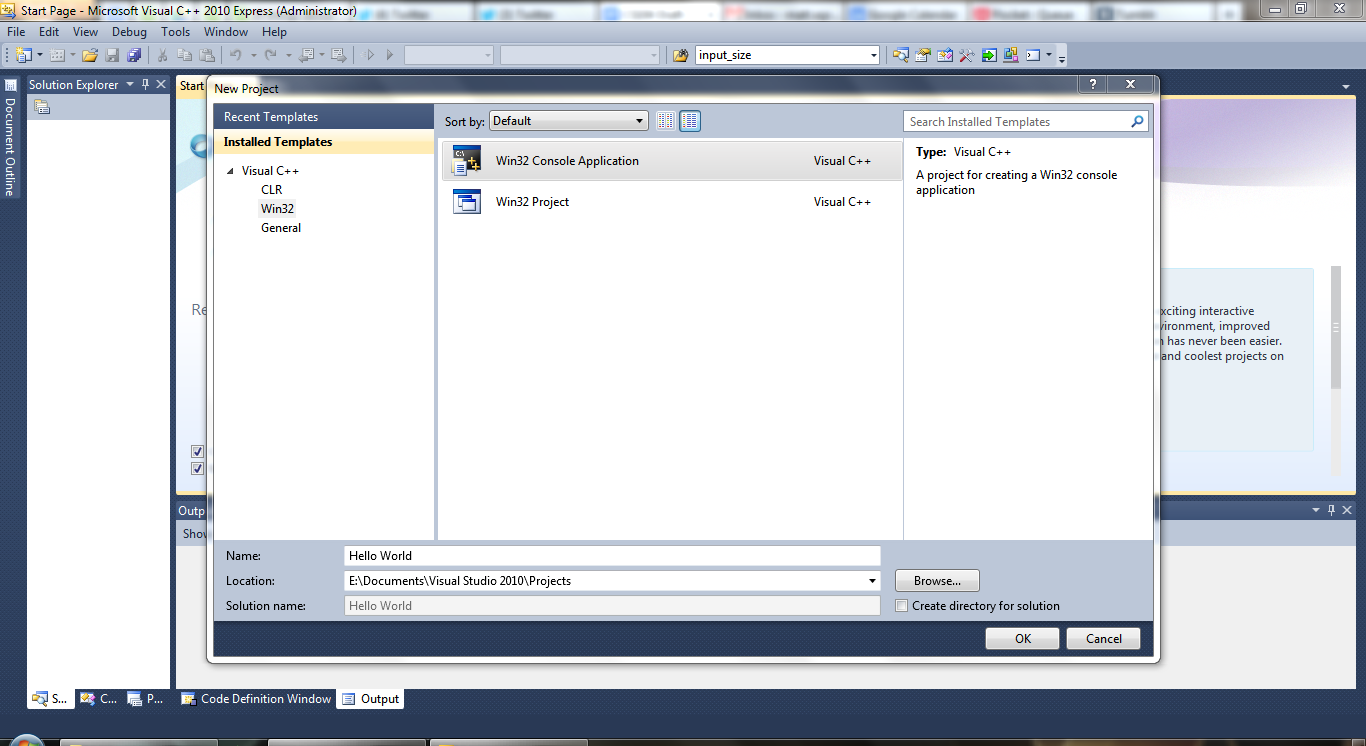
\includegraphics[width=0.47\textwidth]{1.png}
		\caption{Project Creation Dialog Box}
		\label{fig:projcreation}
	\end{figure}
	\item On the Application Settings page under Additional Options, check \texttt{Empty Project}. There should be a message at the bottom that says “Creating project ‘Hello World’… project creation successful.” This will ensure that your program does not have any initial miscellaneous code that could possibly affect the code compilation.
	\begin{figure}[htbp]
		\centering
		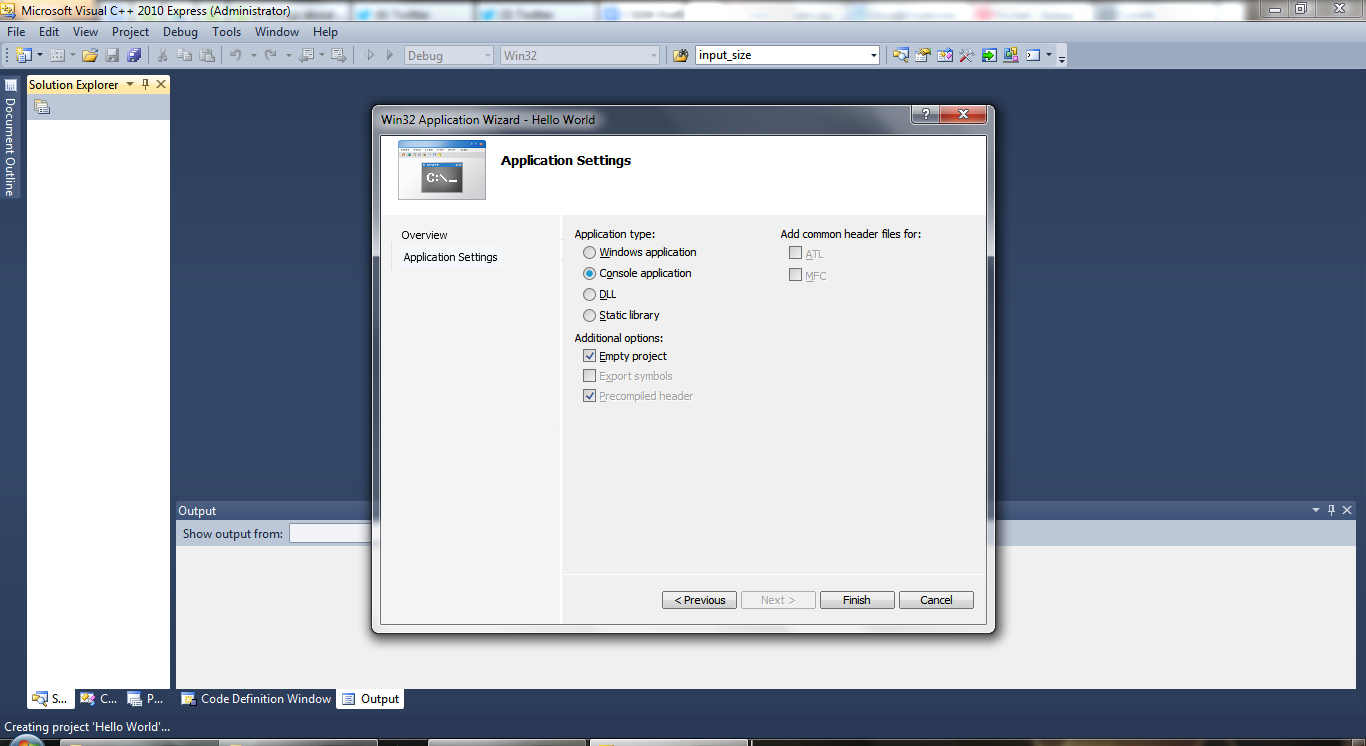
\includegraphics[width=0.47\textwidth]{2.png}
		\caption{Application Settings}
		\label{fig:appsettings}
	\end{figure}
\end{enumerate}

\subsection{Writing Code for your Project}
\begin{enumerate}
	\item Your project will appear on the screen. To begin writing code for your program, you must add a source file. To do so, right click \texttt{Source Files} under your project name. Select \texttt{Add New Item}. 	
	\begin{figure}[htbp]
		\centering
		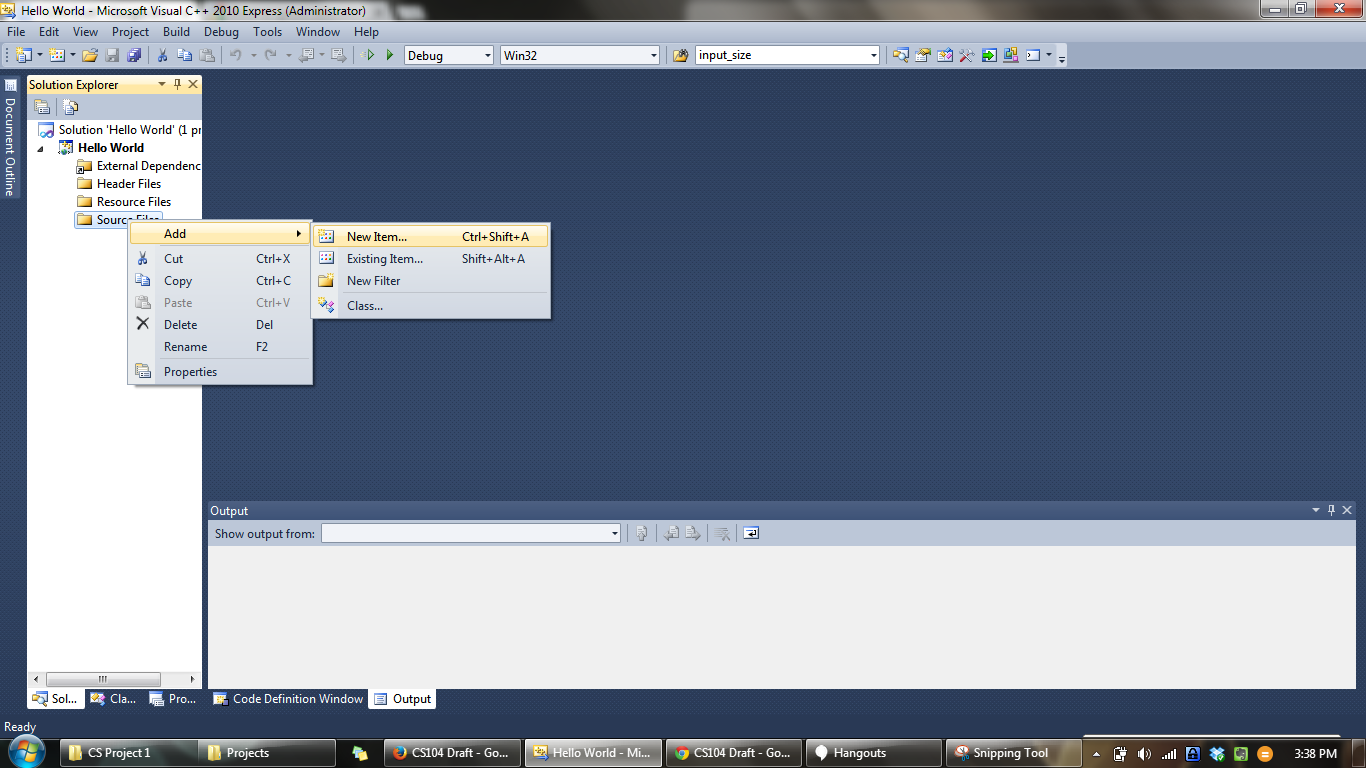
\includegraphics[width=0.47\textwidth]{3.png}
		\caption{Adding a Source File}
		\label{fig:sourcefile}
	\end{figure}
	\item A dialog box will appear. Under Visual C++ on the left side, click \texttt{Code}. Select \texttt{C++ File} and name your source file. Most people use “main” to indicate where the core of the program code sits. 
	\item A blank page will appear. For your main source file, you must include the following lines of code:
	\begin{enumerate}
		\item \texttt{include <iostream>}
	\begin{enumerate}
	  \item This command includes the library where all input and output functions are defined. That way, when the program is being built, the compiler will know what each input and output function means.
	\end{enumerate}	
	  \item \texttt{using namespace std;}
	\begin{enumerate}
	  \item As you will learn in class, a namespace groups items such as objects and classes under a single name.\footnote{\url{http://www.cplusplus.com/doc/tutorial/namespaces/}} The std namespace is used by all files in the C++ library, so it is necessary to include this line of command to avoid having to write std:: before each command.
	\end{enumerate}
	  \item \texttt{int main() \{..your code here.. return 0;\}}
	\begin{enumerate}
	  \item This is where your core program code will sit. The code for the program will be between the curly brackets. At the end of your code, you must return an integer value (usually 0) to instruct the program to stop when it has completed running through the code.
	\end{enumerate}
	\end{enumerate}
	\item To print out a string, use the command cout, followed by \textless \textless. Put the desired string, which is in this case Hello World!, in double quotation marks. 
	\begin{figure}[htbp]
		\centering
		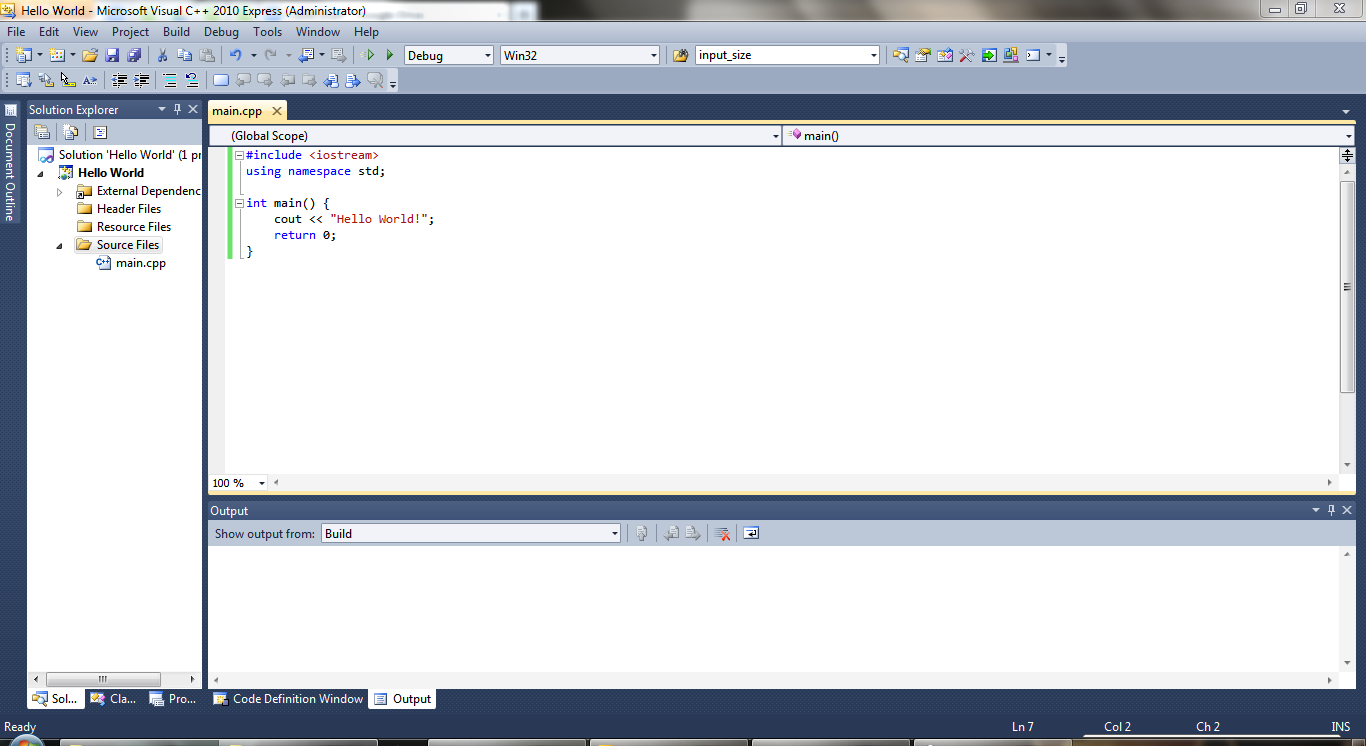
\includegraphics[width=0.47\textwidth]{4.png}
		\caption{Main Source File}
		\label{fig:main}
	\end{figure}
\end{enumerate}
	

\subsection{Building Your Project} To see how your program works, you must build the code. This includes compilation and execution of the project.
\begin{enumerate}
  \item Click on \texttt{Build} at the top of the screen. Select \texttt{Build Solution}. 
  \item If your project compiled successfully, the dialog box at the bottom of the screen will say “Build: 1 succeeded, 0 failed” and a terminal will pop up.
\item If your project did not compile successfully, make sure that all of your syntax is correct (e.g. no missing commas or semicolons). You can also debug your code to see where your program fails to build.
\end{enumerate}

\section{Simple Debugging in Visual Studio} Visual Studio has a built in debugger. A debugger allows you to set break points in your code that will allow you to see where your code may not function the way you intended. When you begin the debugging process for a specific program, the code will execute up until the statement where the break point has been set. The break point statement will not be executed.
\begin{enumerate}
  \item To set a break point, click on the tray on the side. A red bubble should appear where you clicked your mouse. If you right click on the tray, you will see options for different break points. There are several types of break points. One type is a conditional break point, which will stop the program when that condition is true. 
 \begin{figure}[htbp]
		\centering
		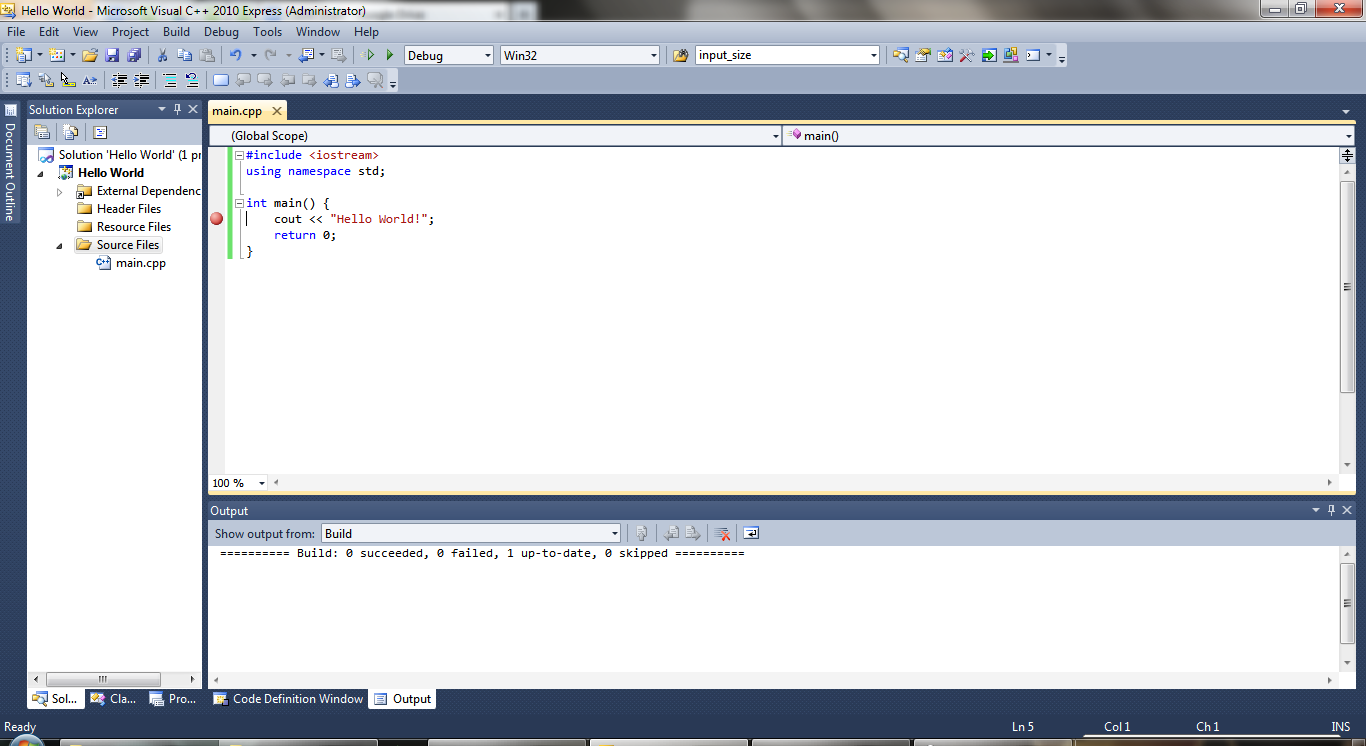
\includegraphics[width=0.47\textwidth]{5.png}
		\caption{Debugging in Visual Studio}
		\label{fig:debug}
	\end{figure}
  \item Right click on your project name, and then select \texttt{Debug}. 
\end{enumerate}
\end{document}